% Options for packages loaded elsewhere
\PassOptionsToPackage{unicode}{hyperref}
\PassOptionsToPackage{hyphens}{url}
%
\documentclass[
]{book}
\title{Métodos Computacionais para Análise Estrutural: Aplicações em Octave e Python}
\author{Paulo de Souza Silva}
\date{2022-02-13}

\usepackage{amsmath,amssymb}
\usepackage{lmodern}
\usepackage{iftex}
\ifPDFTeX
  \usepackage[T1]{fontenc}
  \usepackage[utf8]{inputenc}
  \usepackage{textcomp} % provide euro and other symbols
\else % if luatex or xetex
  \usepackage{unicode-math}
  \defaultfontfeatures{Scale=MatchLowercase}
  \defaultfontfeatures[\rmfamily]{Ligatures=TeX,Scale=1}
\fi
% Use upquote if available, for straight quotes in verbatim environments
\IfFileExists{upquote.sty}{\usepackage{upquote}}{}
\IfFileExists{microtype.sty}{% use microtype if available
  \usepackage[]{microtype}
  \UseMicrotypeSet[protrusion]{basicmath} % disable protrusion for tt fonts
}{}
\makeatletter
\@ifundefined{KOMAClassName}{% if non-KOMA class
  \IfFileExists{parskip.sty}{%
    \usepackage{parskip}
  }{% else
    \setlength{\parindent}{0pt}
    \setlength{\parskip}{6pt plus 2pt minus 1pt}}
}{% if KOMA class
  \KOMAoptions{parskip=half}}
\makeatother
\usepackage{xcolor}
\IfFileExists{xurl.sty}{\usepackage{xurl}}{} % add URL line breaks if available
\IfFileExists{bookmark.sty}{\usepackage{bookmark}}{\usepackage{hyperref}}
\hypersetup{
  pdftitle={Métodos Computacionais para Análise Estrutural: Aplicações em Octave e Python},
  pdfauthor={Paulo de Souza Silva},
  hidelinks,
  pdfcreator={LaTeX via pandoc}}
\urlstyle{same} % disable monospaced font for URLs
\usepackage{color}
\usepackage{fancyvrb}
\newcommand{\VerbBar}{|}
\newcommand{\VERB}{\Verb[commandchars=\\\{\}]}
\DefineVerbatimEnvironment{Highlighting}{Verbatim}{commandchars=\\\{\}}
% Add ',fontsize=\small' for more characters per line
\usepackage{framed}
\definecolor{shadecolor}{RGB}{248,248,248}
\newenvironment{Shaded}{\begin{snugshade}}{\end{snugshade}}
\newcommand{\AlertTok}[1]{\textcolor[rgb]{0.94,0.16,0.16}{#1}}
\newcommand{\AnnotationTok}[1]{\textcolor[rgb]{0.56,0.35,0.01}{\textbf{\textit{#1}}}}
\newcommand{\AttributeTok}[1]{\textcolor[rgb]{0.77,0.63,0.00}{#1}}
\newcommand{\BaseNTok}[1]{\textcolor[rgb]{0.00,0.00,0.81}{#1}}
\newcommand{\BuiltInTok}[1]{#1}
\newcommand{\CharTok}[1]{\textcolor[rgb]{0.31,0.60,0.02}{#1}}
\newcommand{\CommentTok}[1]{\textcolor[rgb]{0.56,0.35,0.01}{\textit{#1}}}
\newcommand{\CommentVarTok}[1]{\textcolor[rgb]{0.56,0.35,0.01}{\textbf{\textit{#1}}}}
\newcommand{\ConstantTok}[1]{\textcolor[rgb]{0.00,0.00,0.00}{#1}}
\newcommand{\ControlFlowTok}[1]{\textcolor[rgb]{0.13,0.29,0.53}{\textbf{#1}}}
\newcommand{\DataTypeTok}[1]{\textcolor[rgb]{0.13,0.29,0.53}{#1}}
\newcommand{\DecValTok}[1]{\textcolor[rgb]{0.00,0.00,0.81}{#1}}
\newcommand{\DocumentationTok}[1]{\textcolor[rgb]{0.56,0.35,0.01}{\textbf{\textit{#1}}}}
\newcommand{\ErrorTok}[1]{\textcolor[rgb]{0.64,0.00,0.00}{\textbf{#1}}}
\newcommand{\ExtensionTok}[1]{#1}
\newcommand{\FloatTok}[1]{\textcolor[rgb]{0.00,0.00,0.81}{#1}}
\newcommand{\FunctionTok}[1]{\textcolor[rgb]{0.00,0.00,0.00}{#1}}
\newcommand{\ImportTok}[1]{#1}
\newcommand{\InformationTok}[1]{\textcolor[rgb]{0.56,0.35,0.01}{\textbf{\textit{#1}}}}
\newcommand{\KeywordTok}[1]{\textcolor[rgb]{0.13,0.29,0.53}{\textbf{#1}}}
\newcommand{\NormalTok}[1]{#1}
\newcommand{\OperatorTok}[1]{\textcolor[rgb]{0.81,0.36,0.00}{\textbf{#1}}}
\newcommand{\OtherTok}[1]{\textcolor[rgb]{0.56,0.35,0.01}{#1}}
\newcommand{\PreprocessorTok}[1]{\textcolor[rgb]{0.56,0.35,0.01}{\textit{#1}}}
\newcommand{\RegionMarkerTok}[1]{#1}
\newcommand{\SpecialCharTok}[1]{\textcolor[rgb]{0.00,0.00,0.00}{#1}}
\newcommand{\SpecialStringTok}[1]{\textcolor[rgb]{0.31,0.60,0.02}{#1}}
\newcommand{\StringTok}[1]{\textcolor[rgb]{0.31,0.60,0.02}{#1}}
\newcommand{\VariableTok}[1]{\textcolor[rgb]{0.00,0.00,0.00}{#1}}
\newcommand{\VerbatimStringTok}[1]{\textcolor[rgb]{0.31,0.60,0.02}{#1}}
\newcommand{\WarningTok}[1]{\textcolor[rgb]{0.56,0.35,0.01}{\textbf{\textit{#1}}}}
\usepackage{longtable,booktabs,array}
\usepackage{calc} % for calculating minipage widths
% Correct order of tables after \paragraph or \subparagraph
\usepackage{etoolbox}
\makeatletter
\patchcmd\longtable{\par}{\if@noskipsec\mbox{}\fi\par}{}{}
\makeatother
% Allow footnotes in longtable head/foot
\IfFileExists{footnotehyper.sty}{\usepackage{footnotehyper}}{\usepackage{footnote}}
\makesavenoteenv{longtable}
\usepackage{graphicx}
\makeatletter
\def\maxwidth{\ifdim\Gin@nat@width>\linewidth\linewidth\else\Gin@nat@width\fi}
\def\maxheight{\ifdim\Gin@nat@height>\textheight\textheight\else\Gin@nat@height\fi}
\makeatother
% Scale images if necessary, so that they will not overflow the page
% margins by default, and it is still possible to overwrite the defaults
% using explicit options in \includegraphics[width, height, ...]{}
\setkeys{Gin}{width=\maxwidth,height=\maxheight,keepaspectratio}
% Set default figure placement to htbp
\makeatletter
\def\fps@figure{htbp}
\makeatother
\setlength{\emergencystretch}{3em} % prevent overfull lines
\providecommand{\tightlist}{%
  \setlength{\itemsep}{0pt}\setlength{\parskip}{0pt}}
\setcounter{secnumdepth}{5}
\usepackage{booktabs}
\usepackage[utf8]{inputenc}
\usepackage[brazil]{babel}
\usepackage[top=2cm, bottom = 3cm,left = 2.5cm,right = 2.5cm]{geometry}
\usepackage{xcolor}

\newtheorem{theorem}{Teorema}
\ifLuaTeX
  \usepackage{selnolig}  % disable illegal ligatures
\fi
\usepackage[]{natbib}
\bibliographystyle{plainnat}

\begin{document}
\maketitle

{
\setcounter{tocdepth}{1}
\tableofcontents
}
\hypertarget{motivauxe7uxe3o}{%
\chapter*{Motivação}\label{motivauxe7uxe3o}}
\addcontentsline{toc}{chapter}{Motivação}

Este livro tem como objetivo ser um material auxiliar para os alunos da disciplina de \textbf{Métodos Computacionais para Análise Estrutural} do curso de \textbf{Engenharia Aeroespacial} da \textbf{Universidade Federal do ABC}. No entanto, o mesmo, tenta abordar de forma clara e concisa os temas referentes a \emph{Álgebra Linear, Cálculo Numério} e \emph{Modelagens Estruturais} para todos aqueles que são intusiastas nesses tópicos.

\hypertarget{por-que-ler-este-livro}{%
\section*{Por que ler este livro?}\label{por-que-ler-este-livro}}
\addcontentsline{toc}{section}{Por que ler este livro?}

\hypertarget{sobre-os-autores}{%
\section*{Sobre os Autores}\label{sobre-os-autores}}
\addcontentsline{toc}{section}{Sobre os Autores}

\emph{Paulo de Souza} é graduando do curso de Engenharia Aeroespacial. Seus interesses são nas áreas de simulação estrutural de aeronaves e aprendizado de máquina com aplicação em frentes da engenharia mecânica.

\hypertarget{part-conhecendo-o-octave-e-o-python}{%
\part{Conhecendo o Octave e o Python}\label{part-conhecendo-o-octave-e-o-python}}

\hypertarget{introduuxe7uxe3o-ao-octave}{%
\chapter{Introdução ao Octave}\label{introduuxe7uxe3o-ao-octave}}

O GNU Octave, ou simplesmente Octave, é um \emph{software} livre para execução e desenvolvimento de operações matemáticas.

\hypertarget{comandos-buxe1sicos-em-octave}{%
\section{Comandos Básicos em Octave}\label{comandos-buxe1sicos-em-octave}}

\hypertarget{operauxe7uxf5es-matemuxe1ticas-e-luxf3gicas}{%
\subsection{Operações Matemáticas e Lógicas}\label{operauxe7uxf5es-matemuxe1ticas-e-luxf3gicas}}

As operações matemáticas simples, adição, subtração, multiplicação e divisão podem ser executadas de maneira direta, como é apresentado na sequência

\begin{Shaded}
\begin{Highlighting}[]
\FloatTok{2} \OperatorTok{+} \FloatTok{5}
\FloatTok{2} \OperatorTok{{-}} \FloatTok{5}
\FloatTok{2} \OperatorTok{*} \FloatTok{5}
\FloatTok{2} \OperatorTok{/} \FloatTok{5}
\end{Highlighting}
\end{Shaded}

\begin{verbatim}
## ans = 7
## ans = -3
## ans = 10
## ans = 0.4000
\end{verbatim}

\hypertarget{vetores-e-matrizes}{%
\subsection{Vetores e Matrizes}\label{vetores-e-matrizes}}

Esta é uma forma de montar uma matriz \(3 \times 3\) em \textbf{Octave}

\begin{Shaded}
\begin{Highlighting}[]
\NormalTok{A }\OperatorTok{=}\NormalTok{ [}\FloatTok{1} \FloatTok{2} \FloatTok{3}\OperatorTok{;}\FloatTok{4} \FloatTok{5} \FloatTok{6}\OperatorTok{;}\FloatTok{7} \FloatTok{8} \FloatTok{9}\NormalTok{]}
\end{Highlighting}
\end{Shaded}

\begin{verbatim}
## A =
## 
##    1   2   3
##    4   5   6
##    7   8   9
\end{verbatim}

Existem alguns comandos que automatizam a criação de algumas matrizes; em algumas ocasiões serão necessárias o uso de \textbf{matrizes de zeros} ou da \textbf{matriz identidade}, os comandos para elaborar ambas são respectivamente:

\begin{Shaded}
\begin{Highlighting}[]
\NormalTok{A }\OperatorTok{=} \FunctionTok{zeros}\NormalTok{(}\FloatTok{3}\OperatorTok{,}\FloatTok{3}\NormalTok{) }\CommentTok{\%matriz de zeros de dimensao 3 por 3}
\end{Highlighting}
\end{Shaded}

\begin{verbatim}
## A =
## 
##    0   0   0
##    0   0   0
##    0   0   0
\end{verbatim}

\begin{Shaded}
\begin{Highlighting}[]
\NormalTok{A }\OperatorTok{=} \FunctionTok{eye}\NormalTok{(}\FloatTok{3}\OperatorTok{,}\FloatTok{3}\NormalTok{) }\CommentTok{\%matriz identidade de dimensao 3 por 3}
\end{Highlighting}
\end{Shaded}

\begin{verbatim}
## A =
## 
## Diagonal Matrix
## 
##    1   0   0
##    0   1   0
##    0   0   1
\end{verbatim}

\hypertarget{gruxe1ficos}{%
\subsection{Gráficos}\label{gruxe1ficos}}

Para gerar o gráficos bidimensionais, define-se os valores do eixo X e depois aplica-se a equação desejada; por exemplo, para \(y = x^2 | \ x \in [-5,5]\) pode ser feito

\begin{Shaded}
\begin{Highlighting}[]
\NormalTok{x }\OperatorTok{=} \OperatorTok{{-}}\FloatTok{5}\OperatorTok{:}\FloatTok{0.1}\OperatorTok{:}\FloatTok{5}\OperatorTok{;}
\NormalTok{y }\OperatorTok{=}\NormalTok{ x}\OperatorTok{.\^{}}\FloatTok{2}\OperatorTok{;}

\FunctionTok{plot}\NormalTok{(x}\OperatorTok{,}\NormalTok{y}\OperatorTok{,}\StringTok{\textquotesingle{}r{-}\textquotesingle{}}\NormalTok{)}
\FunctionTok{grid}\NormalTok{ on}
\FunctionTok{print} \OperatorTok{{-}}\NormalTok{djpg parabola.jpg}
\end{Highlighting}
\end{Shaded}

\begin{quote}
\textbf{OBS:} O comando \texttt{print\ -djpg\ parabola.jpg} não é necessário no Octave, os autores o deixaram no corpo do código apenas para salvar a imagem e assim aplica-lá ao livro.
\end{quote}

\begin{figure}

{\centering 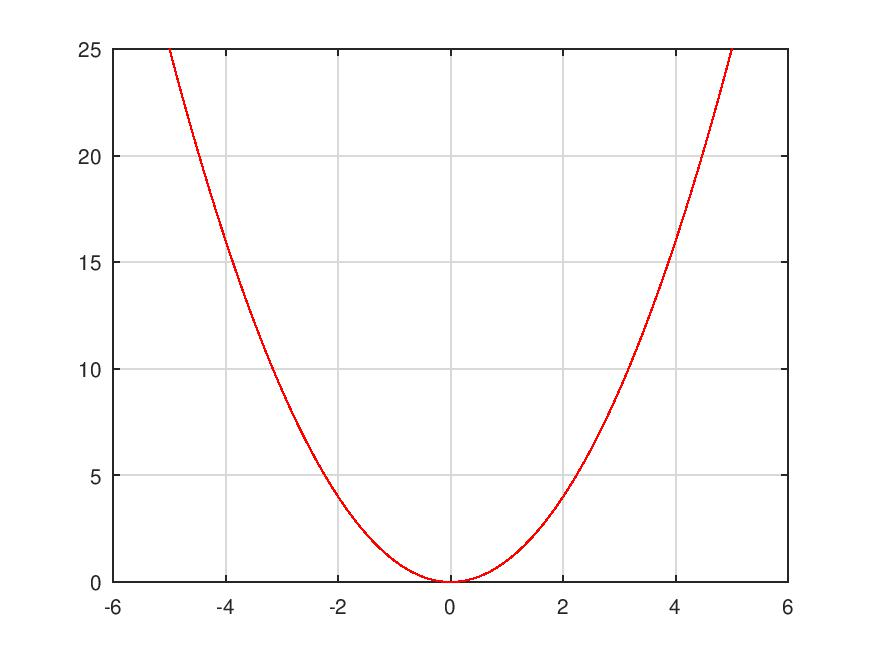
\includegraphics[width=0.5\linewidth]{parabola} 

}

\caption{Parábola definida de -5 à 5}\label{fig:unnamed-chunk-6}
\end{figure}

\hypertarget{programauxe7uxe3o-em-octave}{%
\section{Programação em Octave}\label{programauxe7uxe3o-em-octave}}

\hypertarget{estruturas-de-repetiuxe7uxe3o}{%
\subsection{Estruturas de Repetição}\label{estruturas-de-repetiuxe7uxe3o}}

\hypertarget{funuxe7uxf5es-function}{%
\subsection{\texorpdfstring{Funções \emph{function}}{Funções function}}\label{funuxe7uxf5es-function}}

\begin{Shaded}
\begin{Highlighting}[]
\ControlFlowTok{function} \BuiltInTok{I} \OperatorTok{=}\NormalTok{ InerciaRet(h}\OperatorTok{,}\NormalTok{b)}
\CommentTok{\% Momento de Inercia de uma barra de seção retangular}
\CommentTok{\% h {-} altura da seção}
\CommentTok{\% b {-} base da seção}

\BuiltInTok{I} \OperatorTok{=}\NormalTok{ h}\OperatorTok{\^{}}\FloatTok{3}\OperatorTok{*}\NormalTok{b}\OperatorTok{/}\FloatTok{12}
\end{Highlighting}
\end{Shaded}

É possível então chamar a função pela \emph{Janela de Comandos} ou de outro \emph{script}

\begin{verbatim}
altura = 2;
base = 3;
I = InericaRet(altura,base)
\end{verbatim}

\begin{verbatim}
## I = 
##
##   2
\end{verbatim}

\hypertarget{leitura-de-documentos-externos}{%
\subsection{Leitura de documentos externos}\label{leitura-de-documentos-externos}}

\hypertarget{bibliotecas}{%
\subsection{Bibliotecas}\label{bibliotecas}}

Existem diversas bibliotecas extras no Octave, aqui serão apresentadas apenas duas que por ventura são utilizadas ao decorrer do livro, para mais detalhes consulte\ldots{}

\hypertarget{cross}{%
\chapter{Introdução ao Python}\label{cross}}

\hypertarget{comandos-buxe1sicos-em-python}{%
\section{Comandos Básicos em Python}\label{comandos-buxe1sicos-em-python}}

Esta é uma forma de montar uma matriz \(3 \times 3\) em \textbf{Python}

\begin{Shaded}
\begin{Highlighting}[]
\CommentTok{\#Matriz 3x3}
\ImportTok{import}\NormalTok{ numpy }\ImportTok{as}\NormalTok{ np}

\NormalTok{M }\OperatorTok{=}\NormalTok{ np.array([[}\DecValTok{1}\NormalTok{,}\DecValTok{2}\NormalTok{,}\DecValTok{3}\NormalTok{],}
\NormalTok{              [}\DecValTok{4}\NormalTok{,}\DecValTok{5}\NormalTok{,}\DecValTok{6}\NormalTok{],}
\NormalTok{              [}\DecValTok{7}\NormalTok{,}\DecValTok{8}\NormalTok{,}\DecValTok{9}\NormalTok{]])}
\BuiltInTok{print}\NormalTok{(M)}
\end{Highlighting}
\end{Shaded}

\begin{verbatim}
## [[1 2 3]
##  [4 5 6]
##  [7 8 9]]
\end{verbatim}

\hypertarget{part-resoluuxe7uxe3o-de-sistemas-e-aproximauxe7uxe3o-de-funuxe7uxf5es}{%
\part{Resolução de Sistemas e Aproximação de Funções}\label{part-resoluuxe7uxe3o-de-sistemas-e-aproximauxe7uxe3o-de-funuxe7uxf5es}}

\hypertarget{sistemas-de-equauxe7uxf5es}{%
\chapter{Sistemas de Equações}\label{sistemas-de-equauxe7uxf5es}}

\hypertarget{equauxe7uxf5es-nuxe3o-lineares}{%
\section{Equações Não-Lineares}\label{equauxe7uxf5es-nuxe3o-lineares}}

\hypertarget{muxe9todo-de-newton}{%
\subsection{Método de Newton}\label{muxe9todo-de-newton}}

\hypertarget{muxe9todo-das-secantes}{%
\subsection{Método das Secantes}\label{muxe9todo-das-secantes}}

\hypertarget{muxe9todo-de-regula-falsi}{%
\subsection{Método de Regula Falsi}\label{muxe9todo-de-regula-falsi}}

\hypertarget{sistemas-de-equauxe7uxf5es-nuxe3o-lineares}{%
\subsection{Sistemas de Equações não lineares}\label{sistemas-de-equauxe7uxf5es-nuxe3o-lineares}}

\hypertarget{equauxe7uxf5es-polinomiais}{%
\subsection{Equações Polinomiais}\label{equauxe7uxf5es-polinomiais}}

\hypertarget{soluuxe7uxe3o-de-equauxe7uxf5es-lineares-muxe9todos-exatos}{%
\section{Solução de Equações Lineares: Métodos Exatos}\label{soluuxe7uxe3o-de-equauxe7uxf5es-lineares-muxe9todos-exatos}}

\hypertarget{decomposiuxe7uxe3o-lu}{%
\subsection{Decomposição LU}\label{decomposiuxe7uxe3o-lu}}

\hypertarget{eliminauxe7uxe3o-de-gauss}{%
\subsection{Eliminação de Gauss}\label{eliminauxe7uxe3o-de-gauss}}

\hypertarget{decomposiuxe7uxe3o-de-cholesky}{%
\subsection{Decomposição de Cholesky}\label{decomposiuxe7uxe3o-de-cholesky}}

Se uma matriz \textbf{A} for \textbf{simétrica} e \textbf{positiva definida}, então A pode ser decomposta da forma:
\[A = GG^T\]

\begin{itemize}
\tightlist
\item
  \textbf{Matriz Simétrica}
\end{itemize}

\begin{quote}
Uma matriz simétrica é aquela no qual suas componentes \(a_{i,j}\) tem valores iguais as componentes \(a_{j,i}\), isto é:
\end{quote}

\[a_{i,j} = a_{j,i}\]

\begin{itemize}
\tightlist
\item
  \textbf{Matriz Positiva Definida}
\end{itemize}

\begin{quote}
Uma matriz é dita positiva definida se ocorre um dos seguintes fatos:\\
1. Os autovalores de A são todos positivos\\
2. Os menores principais são positivos\\
3. \(v^TAv > 0, \forall v \neq 0\)
\end{quote}

Abaixo um o teorema \ref{thm:cho} define o método para execução de Cholesky

\begin{theorem}
\protect\hypertarget{thm:cho}{}\label{thm:cho}Se uma matriz \textbf{A} for \textbf{simétrica} e \textbf{positiva definida}, então \emph{existe uma única} matriz triangular G, com elementos diagonais positivos tal que \(A = GG^T\).
\end{theorem}

Isto é, para um caso \(3 \times 3\) é possível representar

\[\begin{pmatrix} 
a_{11} & a_{12} & a_{13} \\
a_{21} & a_{22} & a_{23} \\
a_{31} & a_{32} & a_{33} 
\end{pmatrix} = 
\begin{pmatrix}
g_{11} & 0 & 0 \\
g_{21} & g_{22} & 0 \\
g_{31} & g_{32} & g_{33} 
\end{pmatrix}
\begin{pmatrix}
g_{11} & g_{21} & g_{31} \\
0 & g_{22} & g_{32} \\
0 & 0 & g_{33} 
\end{pmatrix}
\]
Para encontrar os coeficientes da matriz G, é então feito os seguintes processos

\[
g_{11} = \sqrt{a_{11}} \tag{i}\\
\]
\[
g_{i1} = \frac{a_{i1}}{q_{11}} \tag{ii}\\
\]
\[
g_{ii} = \left(a_{ii} - \sum_{k=1}^{i-1} g_{ik}^2 \right)^{1/2} \tag{iii}\\
\]
\[
g_{ij} = \frac{\left(a_{ij} - \sum_{k=1}^{j-1} g_{ik}g_{jk} \right)}{g_{jj}} \tag{iv}
\]
Os passos (iii) e (iv) devem ser intercalados, vista a depedência dos fatores de uma equação na outra, desta forma é indicado o cálculo do valor da diagonal principal e os valores abaixo deste.

Por exemplo, após calcular a componente \(g_{22}\) calcular as demais componentes da coluna 2 (pelo passo iv), e somente ao término deste, ir para a componente \(g_{33}\).

\hypertarget{funuxe7uxe3o-de-cholesky-python}{%
\subsubsection{Função de Cholesky (Python)}\label{funuxe7uxe3o-de-cholesky-python}}

\begin{Shaded}
\begin{Highlighting}[]
\ImportTok{import}\NormalTok{ numpy }\ImportTok{as}\NormalTok{ np}

\CommentTok{\#Funcao que verifica a simetria}
\KeywordTok{def}\NormalTok{ simetrica(U):}
  \ControlFlowTok{for}\NormalTok{ i }\KeywordTok{in} \BuiltInTok{range}\NormalTok{(}\BuiltInTok{len}\NormalTok{(U)):}
    \ControlFlowTok{for}\NormalTok{ j  }\KeywordTok{in} \BuiltInTok{range}\NormalTok{(}\BuiltInTok{len}\NormalTok{(U[}\DecValTok{0}\NormalTok{])):}
      \ControlFlowTok{if}\NormalTok{ U[i][j] }\OperatorTok{!=}\NormalTok{ U[j][i]:}
        \ControlFlowTok{return} \DecValTok{0}
  \ControlFlowTok{return} \DecValTok{1}

\CommentTok{\#Funcao que verifica se a matriz é positiva definida}
\KeywordTok{def}\NormalTok{ pos\_def(U):}
\NormalTok{  auval,auvec }\OperatorTok{=}\NormalTok{ np.linalg.eig(U)}
\NormalTok{  cont }\OperatorTok{=} \DecValTok{0}\OperatorTok{;}
  \ControlFlowTok{for}\NormalTok{ i }\KeywordTok{in} \BuiltInTok{range}\NormalTok{(}\BuiltInTok{len}\NormalTok{(auval)):}
    \ControlFlowTok{if}\NormalTok{ auval[i]}\OperatorTok{\textgreater{}}\DecValTok{0}\NormalTok{:}
\NormalTok{      cont }\OperatorTok{=}\NormalTok{ cont}\OperatorTok{+}\DecValTok{1}
  \ControlFlowTok{if}\NormalTok{ cont }\OperatorTok{==} \BuiltInTok{len}\NormalTok{(U):}
    \ControlFlowTok{return} \DecValTok{1}
  \ControlFlowTok{return} \DecValTok{0}

\CommentTok{\#Funcao que faz a soma para os termos G[i][i]}
\KeywordTok{def}\NormalTok{ SomaCho1(U,i):}
\NormalTok{  soma1 }\OperatorTok{=} \DecValTok{0}
  \ControlFlowTok{for}\NormalTok{ k }\KeywordTok{in} \BuiltInTok{range}\NormalTok{(}\DecValTok{0}\NormalTok{,i):}
\NormalTok{    soma1 }\OperatorTok{=}\NormalTok{ soma1 }\OperatorTok{+}\NormalTok{ np.power(U[i][k],}\DecValTok{2}\NormalTok{)}
  \ControlFlowTok{return}\NormalTok{ soma1}

\CommentTok{\#Funcao que faz a soma para os termos G[i][j]}
\KeywordTok{def}\NormalTok{ SomaCho2(U,i,j):}
\NormalTok{  soma2 }\OperatorTok{=} \DecValTok{0}
  \ControlFlowTok{for}\NormalTok{ k }\KeywordTok{in} \BuiltInTok{range}\NormalTok{(}\DecValTok{0}\NormalTok{,j):}
\NormalTok{    soma2 }\OperatorTok{=}\NormalTok{ soma2 }\OperatorTok{+}\NormalTok{ U[i][k]}\OperatorTok{*}\NormalTok{U[j][k]}
  \ControlFlowTok{return}\NormalTok{ soma2}

\CommentTok{\#Funcao para o Calculo da Decomposicao de Cholesky}
\KeywordTok{def}\NormalTok{ MeuCholesly(A):}
\NormalTok{  G }\OperatorTok{=}\NormalTok{ np.zeros((}\BuiltInTok{len}\NormalTok{(A),}\BuiltInTok{len}\NormalTok{(A)))}
  \ControlFlowTok{if}\NormalTok{ simetrica(A) }\OperatorTok{==}\NormalTok{ pos\_def(A):}
\NormalTok{    G[}\DecValTok{0}\NormalTok{][}\DecValTok{0}\NormalTok{] }\OperatorTok{=}\NormalTok{ np.sqrt(A[}\DecValTok{0}\NormalTok{][}\DecValTok{0}\NormalTok{])}
    \ControlFlowTok{for}\NormalTok{ i }\KeywordTok{in} \BuiltInTok{range}\NormalTok{(}\DecValTok{1}\NormalTok{,}\BuiltInTok{len}\NormalTok{(A)):}
\NormalTok{      G[i][}\DecValTok{0}\NormalTok{] }\OperatorTok{=}\NormalTok{ A[i][}\DecValTok{0}\NormalTok{]}\OperatorTok{/}\NormalTok{G[}\DecValTok{0}\NormalTok{][}\DecValTok{0}\NormalTok{]}
    
    \ControlFlowTok{for}\NormalTok{ j }\KeywordTok{in} \BuiltInTok{range}\NormalTok{(}\DecValTok{1}\NormalTok{,}\BuiltInTok{len}\NormalTok{(A)):}
      \ControlFlowTok{for}\NormalTok{ i }\KeywordTok{in} \BuiltInTok{range}\NormalTok{(j,}\BuiltInTok{len}\NormalTok{(A)):}
        \ControlFlowTok{if}\NormalTok{ i}\OperatorTok{==}\NormalTok{j:}
\NormalTok{          G[i][j] }\OperatorTok{=}\NormalTok{ np.sqrt(A[i][i] }\OperatorTok{{-}}\NormalTok{ SomaCho1(G,i))}
          \CommentTok{\#print(SomaCho1(G,i))}
        \ControlFlowTok{else}\NormalTok{:}
\NormalTok{          G[i][j] }\OperatorTok{=}\NormalTok{ (A[i][j] }\OperatorTok{{-}}\NormalTok{ SomaCho2(G,i,j))}\OperatorTok{/}\NormalTok{G[j][j]}
          \CommentTok{\#print(SomaCho2(G,i,j))}
\NormalTok{    G }\OperatorTok{=}\NormalTok{ np.}\BuiltInTok{round}\NormalTok{(G,}\DecValTok{4}\NormalTok{)}
    \ControlFlowTok{return}\NormalTok{ G }
  \ControlFlowTok{else}\NormalTok{:}
    \ControlFlowTok{return} \BuiltInTok{print}\NormalTok{(}\StringTok{\textquotesingle{}Não é possível usar Decomposição de Cholesky\textquotesingle{}}\NormalTok{)}
\end{Highlighting}
\end{Shaded}

Exemplo matriz \(3 \times 3\)

\begin{Shaded}
\begin{Highlighting}[]

\NormalTok{A }\OperatorTok{=}\NormalTok{ np.array([[}\DecValTok{6}\NormalTok{,}\DecValTok{15}\NormalTok{,}\DecValTok{55}\NormalTok{],}
\NormalTok{              [}\DecValTok{15}\NormalTok{,}\DecValTok{55}\NormalTok{,}\DecValTok{225}\NormalTok{],}
\NormalTok{              [}\DecValTok{55}\NormalTok{,}\DecValTok{225}\NormalTok{,}\DecValTok{979}\NormalTok{]])}

\NormalTok{MeuCholesly(A)}
\end{Highlighting}
\end{Shaded}

\begin{verbatim}
## array([[ 2.4495,  0.    ,  0.    ],
##        [ 6.1237,  4.1833,  0.    ],
##        [22.4537, 20.9165,  6.1101]])
\end{verbatim}

Exemplo matriz \(4 \times 4\)

\begin{Shaded}
\begin{Highlighting}[]
\NormalTok{M }\OperatorTok{=}\NormalTok{ np.array([[}\DecValTok{9}\NormalTok{,}\DecValTok{0}\NormalTok{,}\OperatorTok{{-}}\DecValTok{27}\NormalTok{,}\DecValTok{18}\NormalTok{],}
\NormalTok{              [}\DecValTok{0}\NormalTok{,}\DecValTok{9}\NormalTok{,}\OperatorTok{{-}}\DecValTok{9}\NormalTok{,}\OperatorTok{{-}}\DecValTok{27}\NormalTok{],}
\NormalTok{              [}\OperatorTok{{-}}\DecValTok{27}\NormalTok{,}\OperatorTok{{-}}\DecValTok{9}\NormalTok{,}\DecValTok{99}\NormalTok{,}\OperatorTok{{-}}\DecValTok{27}\NormalTok{],}
\NormalTok{              [}\DecValTok{18}\NormalTok{,}\OperatorTok{{-}}\DecValTok{27}\NormalTok{,}\OperatorTok{{-}}\DecValTok{27}\NormalTok{,}\DecValTok{121}\NormalTok{]])}

\NormalTok{MeuCholesly(M)}
\end{Highlighting}
\end{Shaded}

\begin{verbatim}
## array([[ 3.,  0.,  0.,  0.],
##        [ 0.,  3.,  0.,  0.],
##        [-9., -3.,  3.,  0.],
##        [ 6., -9.,  0.,  2.]])
\end{verbatim}

\hypertarget{comando-linalg.cholesky}{%
\subsubsection{Comando linalg.Cholesky}\label{comando-linalg.cholesky}}

\hypertarget{soluuxe7uxe3o-de-equauxe7uxf5es-lineares-muxe9todos-iterativos}{%
\section{Solução de Equações Lineares: Métodos Iterativos}\label{soluuxe7uxe3o-de-equauxe7uxf5es-lineares-muxe9todos-iterativos}}

\hypertarget{muxe9todo-de-gauss-seidel}{%
\subsection{Método de Gauss Seidel}\label{muxe9todo-de-gauss-seidel}}

\hypertarget{footnotes-and-citations}{%
\chapter{Footnotes and citations}\label{footnotes-and-citations}}

\hypertarget{footnotes}{%
\section{Footnotes}\label{footnotes}}

Footnotes are put inside the square brackets after a caret \texttt{\^{}{[}{]}}. Like this one \footnote{This is a footnote.}.

\hypertarget{citations}{%
\section{Citations}\label{citations}}

Reference items in your bibliography file(s) using \texttt{@key}.

For example, we are using the \textbf{bookdown} package \citep{R-bookdown} (check out the last code chunk in index.Rmd to see how this citation key was added) in this sample book, which was built on top of R Markdown and \textbf{knitr} \citep{xie2015} (this citation was added manually in an external file book.bib).
Note that the \texttt{.bib} files need to be listed in the index.Rmd with the YAML \texttt{bibliography} key.

The RStudio Visual Markdown Editor can also make it easier to insert citations: \url{https://rstudio.github.io/visual-markdown-editing/\#/citations}

\hypertarget{blocks}{%
\chapter{Blocks}\label{blocks}}

\hypertarget{equauxe7uxf5es}{%
\section{Equações}\label{equauxe7uxf5es}}

Aqui está uma equação.

\begin{equation} 
  f\left(k\right) = \binom{n}{k} p^k\left(1-p\right)^{n-k}
  \label{eq:binom}
\end{equation}

You may refer to using \texttt{\textbackslash{}@ref(eq:binom)}, like see Equation \eqref{eq:binom}.

\hypertarget{theorems-and-proofs}{%
\section{Theorems and proofs}\label{theorems-and-proofs}}

Labeled theorems can be referenced in text using \texttt{\textbackslash{}@ref(thm:tri)}, for example, check out this smart theorem \ref{thm:tri}.

\begin{theorem}
\protect\hypertarget{thm:tri}{}\label{thm:tri}For a right triangle, if \(c\) denotes the \emph{length} of the hypotenuse
and \(a\) and \(b\) denote the lengths of the \textbf{other} two sides, we have
\[a^2 + b^2 = c^2\]
\end{theorem}

Read more here \url{https://bookdown.org/yihui/bookdown/markdown-extensions-by-bookdown.html}.

\hypertarget{callout-blocks}{%
\section{Callout blocks}\label{callout-blocks}}

The R Markdown Cookbook provides more help on how to use custom blocks to design your own callouts: \url{https://bookdown.org/yihui/rmarkdown-cookbook/custom-blocks.html}

\hypertarget{sharing-your-book}{%
\chapter{Sharing your book}\label{sharing-your-book}}

\hypertarget{publishing}{%
\section{Publishing}\label{publishing}}

HTML books can be published online, see: \url{https://bookdown.org/yihui/bookdown/publishing.html}

\hypertarget{pages}{%
\section{404 pages}\label{pages}}

By default, users will be directed to a 404 page if they try to access a webpage that cannot be found. If you'd like to customize your 404 page instead of using the default, you may add either a \texttt{\_404.Rmd} or \texttt{\_404.md} file to your project root and use code and/or Markdown syntax.

\hypertarget{metadata-for-sharing}{%
\section{Metadata for sharing}\label{metadata-for-sharing}}

Bookdown HTML books will provide HTML metadata for social sharing on platforms like Twitter, Facebook, and LinkedIn, using information you provide in the \texttt{index.Rmd} YAML. To setup, set the \texttt{url} for your book and the path to your \texttt{cover-image} file. Your book's \texttt{title} and \texttt{description} are also used.

This \texttt{gitbook} uses the same social sharing data across all chapters in your book- all links shared will look the same.

Specify your book's source repository on GitHub using the \texttt{edit} key under the configuration options in the \texttt{\_output.yml} file, which allows users to suggest an edit by linking to a chapter's source file.

Read more about the features of this output format here:

\url{https://pkgs.rstudio.com/bookdown/reference/gitbook.html}

Or use:

\begin{Shaded}
\begin{Highlighting}[]
\NormalTok{?bookdown}\SpecialCharTok{::}\NormalTok{gitbook}
\end{Highlighting}
\end{Shaded}


  \bibliography{book.bib,packages.bib}

\end{document}
